\documentclass[12pt,twoside]{article}

\usepackage{subfig}
\newcommand{\reporttitle}{417 Advanced Graphics}
\newcommand{\reportauthor}{Jinwei Zhang, Yuan Zhu}
\newcommand{\reporttype}{Coursework} 
\newcommand{\cid}{01540854,01531935}

% include files that load packages and define macros
%%%%%%%%%%%%%%%%%%%%%%%%%%%%%%%%%%%%%%%%%
% University Assignment Title Page 
% LaTeX Template
% Version 1.0 (27/12/12)
%
% This template has been downloaded from:
% http://www.LaTeXTemplates.com
%
% Original author:
% WikiBooks (http://en.wikibooks.org/wiki/LaTeX/Title_Creation)
%
% License:
% CC BY-NC-SA 3.0 (http://creativecommons.org/licenses/by-nc-sa/3.0/)
% 
% Instructions for using this template:
% This title page is capable of being compiled as is. This is not useful for 
% including it in another document. To do this, you have two options: 
%
% 1) Copy/paste everything between \begin{document} and \end{document} 
% starting at \begin{titlepage} and paste this into another LaTeX file where you 
% want your title page.
% OR
% 2) Remove everything outside the \begin{titlepage} and \end{titlepage} and 
% move this file to the same directory as the LaTeX file you wish to add it to. 
% Then add \input{./title_page_1.tex} to your LaTeX file where you want your
% title page.
%
%----------------------------------------------------------------------------------------
%	PACKAGES AND OTHER DOCUMENT CONFIGURATIONS
%----------------------------------------------------------------------------------------
\usepackage{ifxetex}
\usepackage{textpos}
\usepackage{natbib}
\usepackage{kpfonts}
\usepackage[a4paper,hmargin=2.8cm,vmargin=2.0cm,includeheadfoot]{geometry}
\usepackage{ifxetex}
\usepackage{stackengine}
\usepackage{tabularx,longtable,multirow,subfigure,caption}%hangcaption
\usepackage{fncylab} %formatting of labels
\usepackage{fancyhdr}
\usepackage{color}
\usepackage[tight,ugly]{units}
\usepackage{url}
\usepackage{float}
\usepackage[english]{babel}
\usepackage{amsmath}
\usepackage{graphicx}
\usepackage[colorinlistoftodos]{todonotes}
\usepackage{dsfont}
\usepackage{epstopdf} % automatically replace .eps with .pdf in graphics
\usepackage{natbib}
\usepackage{backref}
\usepackage{array}
\usepackage{latexsym}
\usepackage{etoolbox}

\usepackage{enumerate} % for numbering with [a)] format 



\ifxetex
\usepackage{fontspec}
\setmainfont[Scale=.8]{OpenDyslexic-Regular}
\else
\usepackage[pdftex,pagebackref,hypertexnames=false,colorlinks]{hyperref} % provide links in pdf
\hypersetup{pdftitle={},
  pdfsubject={}, 
  pdfauthor={\reportauthor},
  pdfkeywords={}, 
  pdfstartview=FitH,
  pdfpagemode={UseOutlines},% None, FullScreen, UseOutlines
  bookmarksnumbered=true, bookmarksopen=true, colorlinks,
    citecolor=black,%
    filecolor=black,%
    linkcolor=black,%
    urlcolor=black}
\usepackage[all]{hypcap}
\fi

\usepackage{tcolorbox}

% various theorems
\usepackage{ntheorem}
\theoremstyle{break}
\newtheorem{lemma}{Lemma}
\newtheorem{theorem}{Theorem}
\newtheorem{remark}{Remark}
\newtheorem{definition}{Definition}
\newtheorem{proof}{Proof}

% example-environment
\newenvironment{example}[1][]
{ 
\vspace{4mm}
\noindent\makebox[\linewidth]{\rule{\hsize}{1.5pt}}
\textbf{Example #1}\\
}
{ 
\noindent\newline\makebox[\linewidth]{\rule{\hsize}{1.0pt}}
}



%\renewcommand{\rmdefault}{pplx} % Palatino
% \renewcommand{\rmdefault}{put} % Utopia

\ifxetex
\else
\renewcommand*{\rmdefault}{bch} % Charter
\renewcommand*{\ttdefault}{cmtt} % Computer Modern Typewriter
%\renewcommand*{\rmdefault}{phv} % Helvetica
%\renewcommand*{\rmdefault}{iwona} % Avant Garde
\fi

\setlength{\parindent}{0em}  % indentation of paragraph

\setlength{\headheight}{14.5pt}
\pagestyle{fancy}
\fancyfoot[ER,OL]{\thepage}%Page no. in the left on
                                %odd pages and on right on even pages
\fancyfoot[OC,EC]{\sffamily }
\renewcommand{\headrulewidth}{0.1pt}
\renewcommand{\footrulewidth}{0.1pt}
\captionsetup{margin=10pt,font=small,labelfont=bf}


%--- chapter heading

\def\@makechapterhead#1{%
  \vspace*{10\p@}%
  {\parindent \z@ \raggedright %\sffamily
        %{\Large \MakeUppercase{\@chapapp} \space \thechapter}
        %\\
        %\hrulefill
        %\par\nobreak
        %\vskip 10\p@
    \interlinepenalty\@M
    \Huge \bfseries 
    \thechapter \space\space #1\par\nobreak
    \vskip 30\p@
  }}

%---chapter heading for \chapter*  
\def\@makeschapterhead#1{%
  \vspace*{10\p@}%
  {\parindent \z@ \raggedright
    \sffamily
    \interlinepenalty\@M
    \Huge \bfseries  
    #1\par\nobreak
    \vskip 30\p@
  }}
  



% %%%%%%%%%%%%% boxit
\def\Beginboxit
   {\par
    \vbox\bgroup
	   \hrule
	   \hbox\bgroup
		  \vrule \kern1.2pt %
		  \vbox\bgroup\kern1.2pt
   }

\def\Endboxit{%
			      \kern1.2pt
		       \egroup
		  \kern1.2pt\vrule
		\egroup
	   \hrule
	 \egroup
   }	

\newenvironment{boxit}{\Beginboxit}{\Endboxit}
\newenvironment{boxit*}{\Beginboxit\hbox to\hsize{}}{\Endboxit}



\allowdisplaybreaks

\makeatletter
\newcounter{elimination@steps}
\newcolumntype{R}[1]{>{\raggedleft\arraybackslash$}p{#1}<{$}}
\def\elimination@num@rights{}
\def\elimination@num@variables{}
\def\elimination@col@width{}
\newenvironment{elimination}[4][0]
{
    \setcounter{elimination@steps}{0}
    \def\elimination@num@rights{#1}
    \def\elimination@num@variables{#2}
    \def\elimination@col@width{#3}
    \renewcommand{\arraystretch}{#4}
    \start@align\@ne\st@rredtrue\m@ne
}
{
    \endalign
    \ignorespacesafterend
}
\newcommand{\eliminationstep}[2]
{
    \ifnum\value{elimination@steps}>0\leadsto\quad\fi
    \left[
        \ifnum\elimination@num@rights>0
            \begin{array}
            {@{}*{\elimination@num@variables}{R{\elimination@col@width}}
            |@{}*{\elimination@num@rights}{R{\elimination@col@width}}}
        \else
            \begin{array}
            {@{}*{\elimination@num@variables}{R{\elimination@col@width}}}
        \fi
            #1
        \end{array}
    \right]
    & 
    \begin{array}{l}
        #2
    \end{array}
    &%                                    moved second & here
    \addtocounter{elimination@steps}{1}
}
\makeatother

%% Fast macro for column vectors
\makeatletter  
\def\colvec#1{\expandafter\colvec@i#1,,,,,,,,,\@nil}
\def\colvec@i#1,#2,#3,#4,#5,#6,#7,#8,#9\@nil{% 
  \ifx$#2$ \begin{bmatrix}#1\end{bmatrix} \else
    \ifx$#3$ \begin{bmatrix}#1\\#2\end{bmatrix} \else
      \ifx$#4$ \begin{bmatrix}#1\\#2\\#3\end{bmatrix}\else
        \ifx$#5$ \begin{bmatrix}#1\\#2\\#3\\#4\end{bmatrix}\else
          \ifx$#6$ \begin{bmatrix}#1\\#2\\#3\\#4\\#5\end{bmatrix}\else
            \ifx$#7$ \begin{bmatrix}#1\\#2\\#3\\#4\\#5\\#6\end{bmatrix}\else
              \ifx$#8$ \begin{bmatrix}#1\\#2\\#3\\#4\\#5\\#6\\#7\end{bmatrix}\else
                 \PackageError{Column Vector}{The vector you tried to write is too big, use bmatrix instead}{Try using the bmatrix environment}
              \fi
            \fi
          \fi
        \fi
      \fi
    \fi
  \fi 
}  
\makeatother

\robustify{\colvec}

%%% Local Variables: 
%%% mode: latex
%%% TeX-master: "notes"
%%% End: 
 % various packages needed for maths etc.
% quick way of adding a figure
\newcommand{\fig}[3]{
 \begin{center}
 \scalebox{#3}{\includegraphics[#2]{#1}}
 \end{center}
}

%\newcommand*{\point}[1]{\vec{\mkern0mu#1}}
\newcommand{\ci}[0]{\perp\!\!\!\!\!\perp} % conditional independence
\newcommand{\point}[1]{{#1}} % points 
\renewcommand{\vec}[1]{{\boldsymbol{{#1}}}} % vector
\newcommand{\mat}[1]{{\boldsymbol{{#1}}}} % matrix
\newcommand{\R}[0]{\mathds{R}} % real numbers
\newcommand{\Z}[0]{\mathds{Z}} % integers
\newcommand{\N}[0]{\mathds{N}} % natural numbers
\newcommand{\nat}[0]{\mathds{N}} % natural numbers
\newcommand{\Q}[0]{\mathds{Q}} % rational numbers
\ifxetex
\newcommand{\C}[0]{\mathds{C}} % complex numbers
\else
\newcommand{\C}[0]{\mathds{C}} % complex numbers
\fi
\newcommand{\tr}[0]{\text{tr}} % trace
\renewcommand{\d}[0]{\mathrm{d}} % total derivative
\newcommand{\inv}{^{-1}} % inverse
\newcommand{\id}{\mathrm{id}} % identity mapping
\renewcommand{\dim}{\mathrm{dim}} % dimension
\newcommand{\rank}[0]{\mathrm{rk}} % rank
\newcommand{\determ}[1]{\mathrm{det}(#1)} % determinant
\newcommand{\scp}[2]{\langle #1 , #2 \rangle}
\newcommand{\kernel}[0]{\mathrm{ker}} % kernel/nullspace
\newcommand{\img}[0]{\mathrm{Im}} % image
\newcommand{\idx}[1]{{(#1)}}
\DeclareMathOperator*{\diag}{diag}
\newcommand{\E}{\mathds{E}} % expectation
\newcommand{\var}{\mathds{V}} % variance
\newcommand{\gauss}[2]{\mathcal{N}\big(#1,\,#2\big)} % gaussian distribution N(.,.)
\newcommand{\gaussx}[3]{\mathcal{N}\big(#1\,|\,#2,\,#3\big)} % gaussian distribution N(.|.,.)
\newcommand{\gaussBig}[2]{\mathcal{N}\left(#1,\,#2\right)} % see above, but with brackets that adjust to the height of the arguments
\newcommand{\gaussxBig}[3]{\mathcal{N}\left(#1\,|\,#2,\,#3\right)} % see above, but with brackets that adjust to the height of the arguments
\DeclareMathOperator{\cov}{Cov} % covariance (matrix) 
\ifxetex
\renewcommand{\T}[0]{^\top} % transpose
\else
\newcommand{\T}[0]{^\top}
\fi
% matrix determinant
\newcommand{\matdet}[1]{
\left|
\begin{matrix}
#1
\end{matrix}
\right|
}



%%% various color definitions
\definecolor{darkgreen}{rgb}{0,0.6,0}

\newcommand{\blue}[1]{{\color{blue}#1}}
\newcommand{\red}[1]{{\color{red}#1}}
\newcommand{\green}[1]{{\color{darkgreen}#1}}
\newcommand{\orange}[1]{{\color{orange}#1}}
\newcommand{\magenta}[1]{{\color{magenta}#1}}
\newcommand{\cyan}[1]{{\color{cyan}#1}}


% redefine emph
\renewcommand{\emph}[1]{\blue{\bf{#1}}}

% place a colored box around a character
\gdef\colchar#1#2{%
  \tikz[baseline]{%
  \node[anchor=base,inner sep=2pt,outer sep=0pt,fill = #2!20] {#1};
    }%
}%
 % short-hand notation and macros


%%%%%%%%%%%%%%%%%%%%%%%%%%%%

\begin{document}
% front page 
% Last modification: 2016-09-29 (Marc Deisenroth)
\begin{titlepage}

\newcommand{\HRule}{\rule{\linewidth}{0.5mm}} % Defines a new command for the horizontal lines, change thickness here


%----------------------------------------------------------------------------------------
%	LOGO SECTION
%----------------------------------------------------------------------------------------


\includegraphics[width = 4cm]{./figures/imperial}\\[0.5cm] 

\begin{center} % Center remainder of the page

%----------------------------------------------------------------------------------------
%	HEADING SECTIONS
%----------------------------------------------------------------------------------------
\textsc{\LARGE \reporttype}\\[1.5cm] 
\textsc{\Large Imperial College London}\\[0.5cm] 
\textsc{\large Department of Computing}\\[0.5cm] 
%----------------------------------------------------------------------------------------
%	TITLE SECTION
%----------------------------------------------------------------------------------------

\HRule \\[0.4cm]
{ \huge \bfseries \reporttitle}\\ % Title of your document
\HRule \\[1.5cm]
\end{center}
%----------------------------------------------------------------------------------------
%	AUTHOR SECTION
%----------------------------------------------------------------------------------------

%\begin{minipage}{0.4\hsize}
\begin{flushleft} \large
\textit{Author:}\\
\reportauthor~(CID: \cid) % Your name
\end{flushleft}
\vspace{2cm}
\makeatletter
Date: \@date 

\vfill % Fill the rest of the page with whitespace



\makeatother


\end{titlepage}







%%%%%%%%%%%%%%%%%%%%%%%%%%%% Main document
\section{Assemble an HDR Image and tonemap for display}
    this is yuan zhu 's part
    



\section{Implement simple Image Based Lighting}
    In this section, we are given an outdoor (urban) lighting environment in lat-long format (.pfm) we need to create an image m of 511x511 resolution containing a mirror ball sphere lit by the lat-long map. \\\\
    The basic algorithm is shown as follow: 
    \begin{enumerate}[1)]
        \item Creating a circle image of diameter 511, First create a square a square image of length and height 511 then set the pixel outside the circle to be black (RGB 0.0) 
        \item for the pixel inside the circle, calculate the normal vector  $\vec{n}(x,y,z)$
        \item After that calculate the reflection vector by using \\
         \begin{align} 
            \vec r = 2*(\mat{n} * \mat{v})*\mat{n} - \mat{v}. 
        \end{align}
        \item Then, mapping the Cartesian coordinate system to Spherical coordinate system using the equation below:
        \begin{align} 
            \begin{aligned} R & = \sqrt { x ^ { 2 } + y ^ { 2 } + z ^ { 2 } } = 255.5 (Radius)
            \\ \theta & = \arctan \left( \frac { \sqrt { x ^ { 2 } + z ^ { 2 } } } { y } \right) = \arccos \left( \frac { y } { \sqrt { x ^ { 2 } + y ^ { 2 } + z ^ { 2 } } } \right) \\ \phi & = \arctan \left( \frac { x } { z } \right) = \arccos \left( \frac { z } { \sqrt { x ^ { 2 } + z ^ { 2 } } } \right) = \arcsin \left( \frac { x } { \sqrt { x ^ { 2 } + z ^ { 2 } } } \right) \end{aligned}
        \end{align}\\
    \begin{figure}[H]
        \centering % this centers the figure
        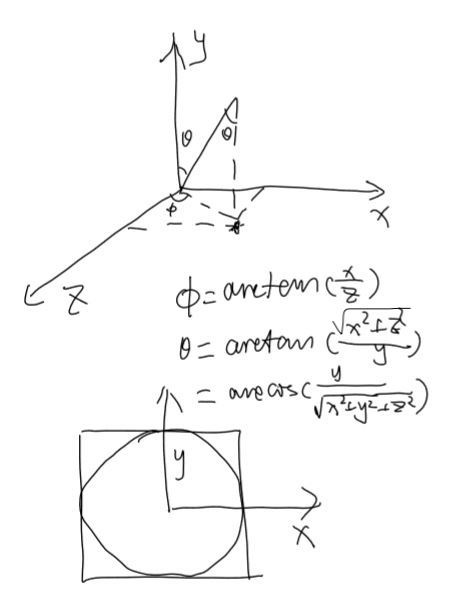
\includegraphics[width=10cm, height=12cm]{./figures/Capture.JPG} % this includes the figure and specifies that it should span 0.7 times the horizontal size of the page
        \caption{This is a draft.} % caption of the figure
        \label{fig:imperial figure} % a label. When we refer to this label from the text, the figure number is included automatically
    \end{figure}
    % Fig.~\ref{fig:imperial figure} shows the Imperial College logo. 
        
        \item Coordinates Y is up, X is pointing right and Z is pointing out of the XY plane. For spherical coordinates of the lat-long map, Width varies along $\phi (0 , 2\pi)$ , and Height varies along $\theta (0 ,\pi)$.
        \item Once we get the vector in spherical coordinates we can map the lat-long map onto the circle using the coordinate system above.
        
        the outcome is as below.
        \begin{figure}[H]
          \centering % this centers the figure
            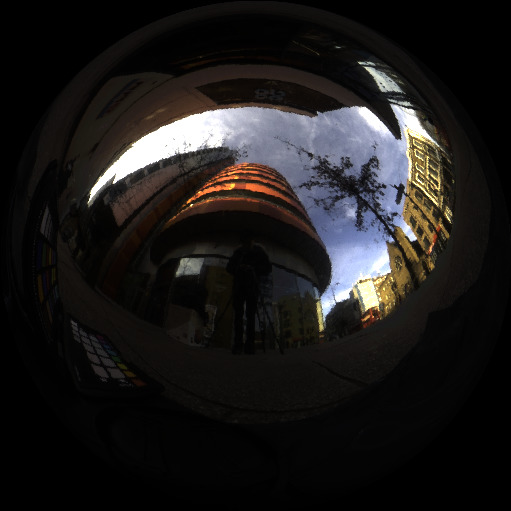
\includegraphics[width= 10cm, height= 10cm]{./figures/result2.jpg} 
            \caption{This is a figure.} % caption of the figure
            \label{fig:imperial figure} % a label. When we refer to this label from the text, the figure number is included automatically
        \end{figure}
        
        \item the gamma correction outcome is: 
        \begin{figure}
            \begin{tabular}{cccc}
            \subfloat[G=1.4 S=3]{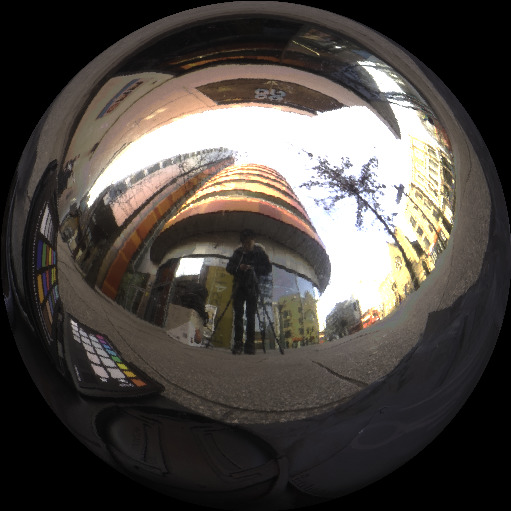
\includegraphics[width = 1.5in]{./figures/result2AfterGamma14Stop3.jpg}} &
            \subfloat[G=1.4 S=5]{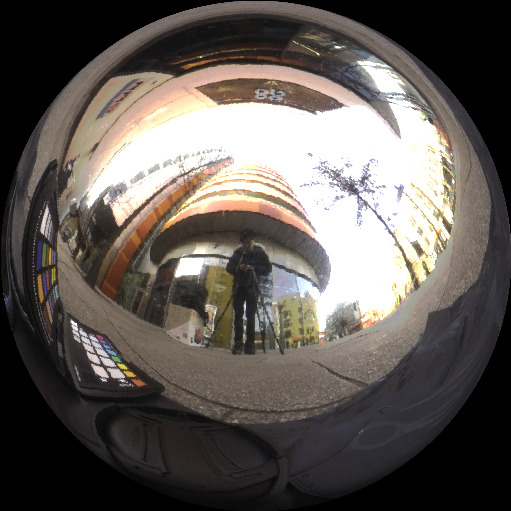
\includegraphics[width = 1.5in]{./figures/result2AfterGamma14Stop5.jpg}} &
            \subfloat[G=1.4 S=7]{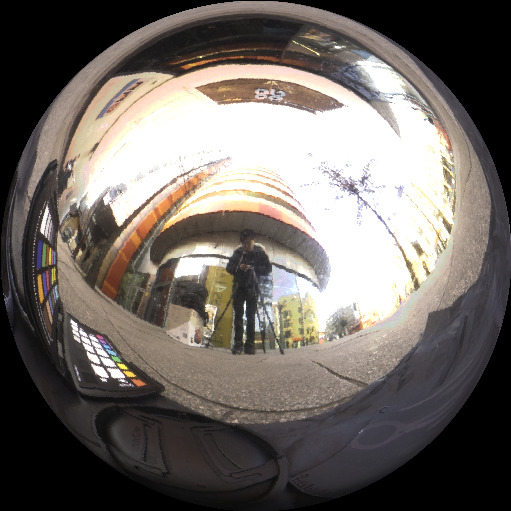
\includegraphics[width = 1.5in]{./figures/result2AfterGamma14Stop7.jpg}} &
            \subfloat[G=1.4 S=9]{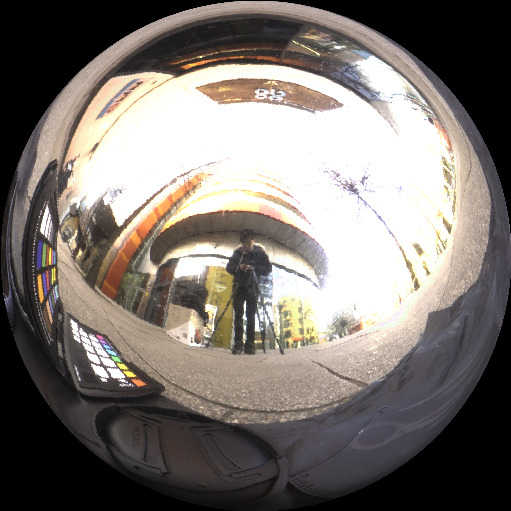
\includegraphics[width = 1.5in]{./figures/result2AfterGamma14Stop9.jpg}}\\
            \subfloat[G=1.8 S=3]{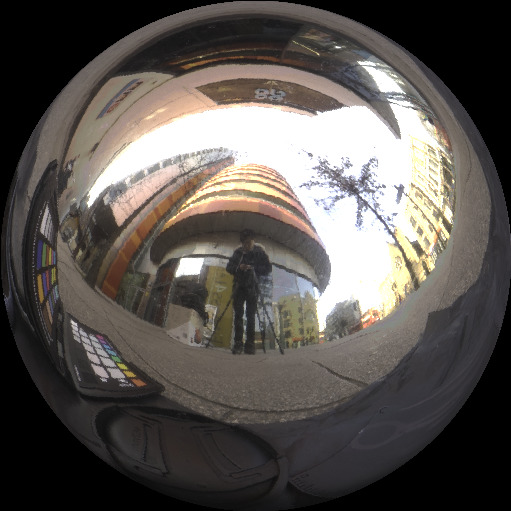
\includegraphics[width = 1.5in]{./figures/result2AfterGamma18Stop3.jpg}} &
            \subfloat[G=1.8 S=5]{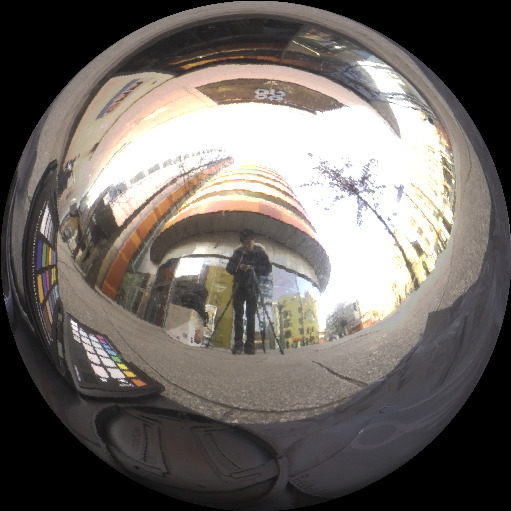
\includegraphics[width = 1.5in]{./figures/result2AfterGamma18Stop5.jpg}} &
            \subfloat[G=1.8 S=7]{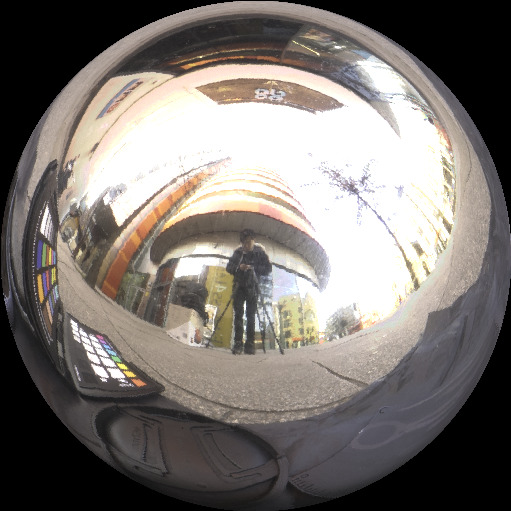
\includegraphics[width = 1.5in]{./figures/result2AfterGamma18Stop7.jpg}} &
            \subfloat[G=1.8 S=9]{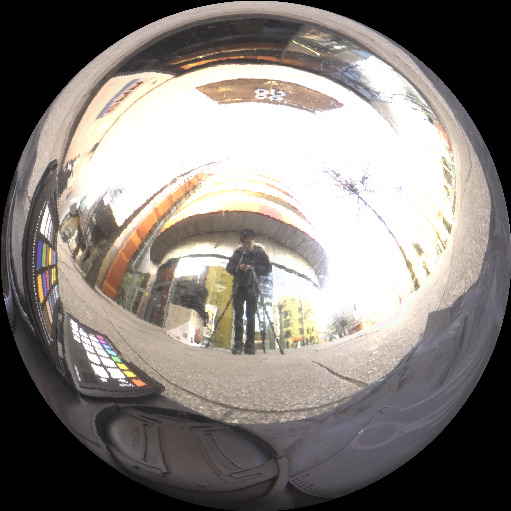
\includegraphics[width = 1.5in]{./figures/result2AfterGamma18Stop9.jpg}}\\
            \subfloat[G=2.2 S=3]{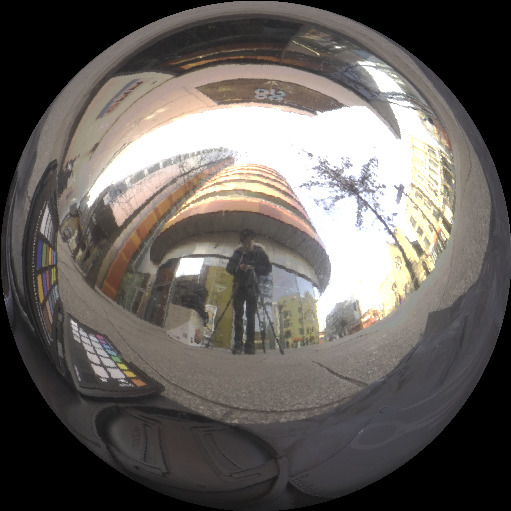
\includegraphics[width = 1.5in]{./figures/result2AfterGamma22Stop3.jpg}} &
            \subfloat[G=2.2 S=5]{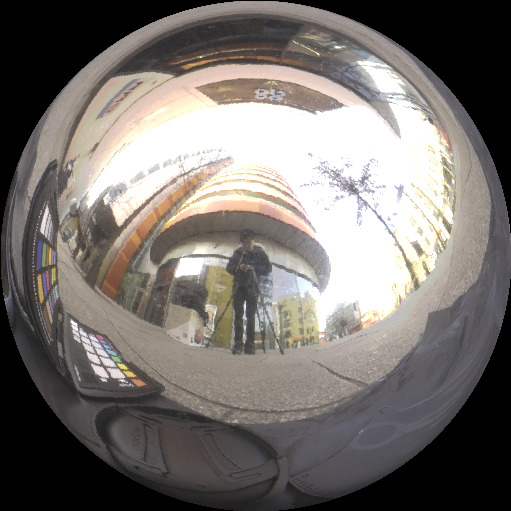
\includegraphics[width = 1.5in]{./figures/result2AfterGamma22Stop5.jpg}} &
            \subfloat[G=2.2 S=7]{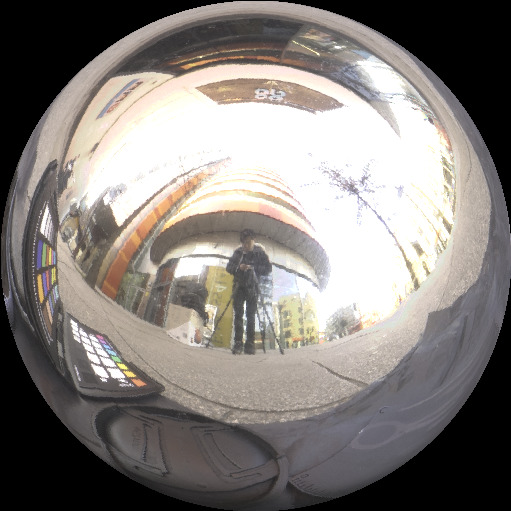
\includegraphics[width = 1.5in]{./figures/result2AfterGamma22Stop7.jpg}} &
            \subfloat[G=2.2 S=9]{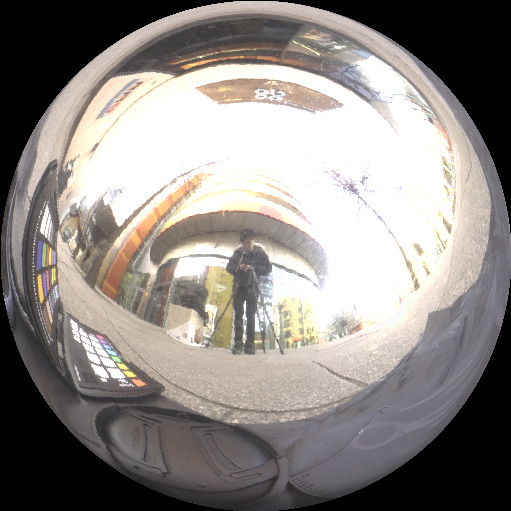
\includegraphics[width = 1.5in]{./figures/result2AfterGamma22Stop9.jpg}}\\
            \subfloat[G=2.6 S=3]{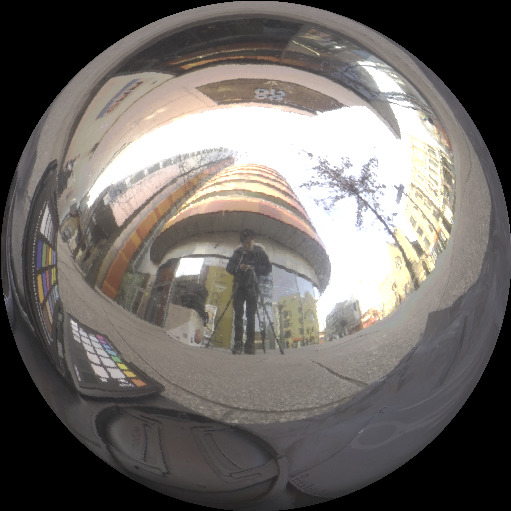
\includegraphics[width = 1.5in]{./figures/result2AfterGamma26Stop3.jpg}} &
            \subfloat[G=2.6 S=5]{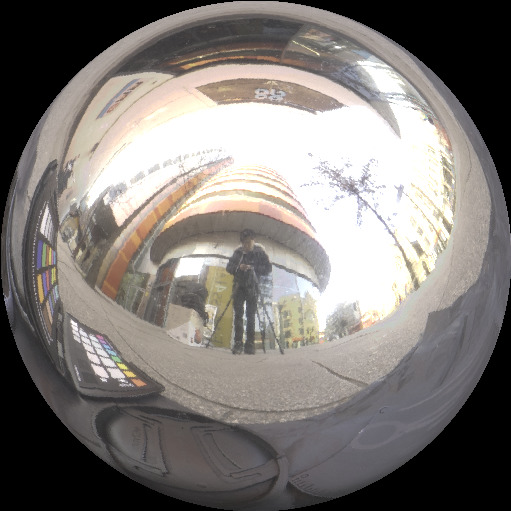
\includegraphics[width = 1.5in]{./figures/result2AfterGamma26Stop5.jpg}} &
            \subfloat[G=2.6 S=7]{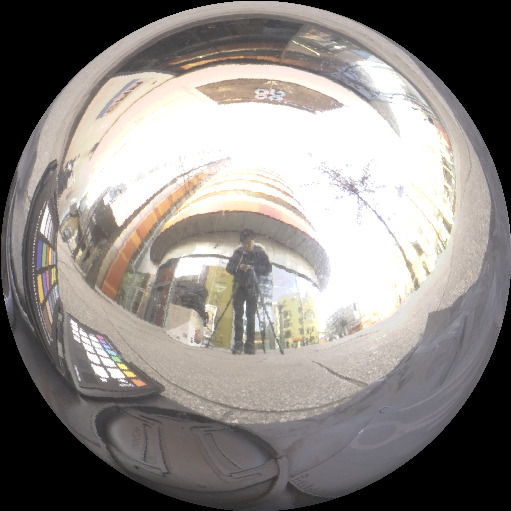
\includegraphics[width = 1.5in]{./figures/result2AfterGamma26Stop7.jpg}} &
            \subfloat[G=2.6 S=9]{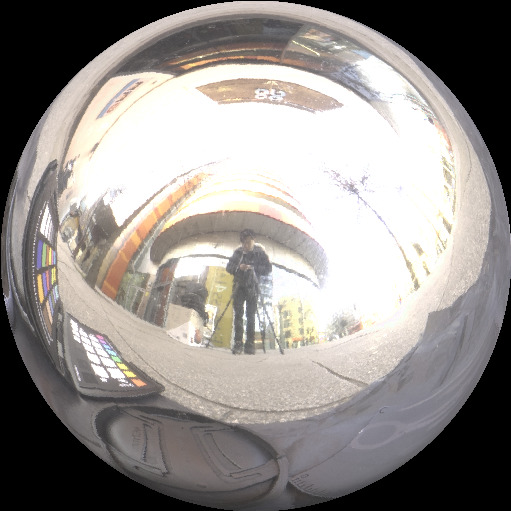
\includegraphics[width = 1.5in]{./figures/result2AfterGamma26Stop9.jpg}}
            \end{tabular}
            \caption{4 x 4}
\end{figure}
        % \\Solution: multiplily C into the function we get\\
        % \begin{align}
        % (\vec x^T -\vec c^T)  \mat C (\vec x - \vec c)+ c_0
        % &=(\vec x^T -\vec c^T)  (\mat C\vec x - \mat C\vec c)+ c_0 \\
        % &=  \vec x^T \mat C\vec x - \vec x^T \mat C\vec c - \vec c^T\mat C\vec x + \vec c^T\mat C\vec c + c_0  \\
        % &=  \vec x^T \mat C\vec x - \vec c^T \mat C\vec x - \vec c^T\mat C\vec x + \vec c^T\mat C\vec c + c_0\\
        %  &=  \vec x^T \mat C\vec x - 2\vec c^T \mat C\vec x + \vec c^T\mat C\vec c + c_0
        % \end{align}
        
        % \begin{align} 
        % f1(x)  &= \vec x^T \vec x + \vec x^T\mat B\vec x  - \vec a^T \vec x + \vec b^T \vec x\\
        % &= \vec x^T (\mat I + \mat B) \vec x   - \vec a^T \vec x + \vec b^T \vec x \\
        % &= \vec x^T (\mat I + \mat B) \vec x   - (\vec a^T - \vec b^T ) \vec x
        % \end{align}
        
        % from (4) and (7) we can get we get \\
        % \begin{align} 
        % \mat I + \mat B = \mat C \\
        % \vec a^T - \vec b^T = 2\vec c^T \mat C\\
        % 0=\vec c^T\mat C\vec c + c_0
        % \end{align}
        
        % \begin{align}
        %     \mat C &= \begin{bmatrix}
        %     4 & -1 \\
        %     -1 & 4 
        %     \end{bmatrix} \\
        %     \vec c &= \begin{bmatrix}
        %         \frac{1}{6} \\
        %         \frac{1}{6} 
        %     \end{bmatrix}\\
        %     c_0 &= -\frac{1}{6} 
        % \end{align}
        
    
    \end{enumerate}
    






\end{document}
%%% Local Variables: 
%%% mode: latex
%%% TeX-master: t
%%% End: 
